% !TEX encoding = UTF-8 Unicode

A linguagem de programação \emph{RNA} apresentada pelo professor é uma linguagem esotérica e nunca utilizada para aplicações práticas, criada em 2008 e implementada em 2011 por Cyrus H.  

Ela possui 16 instruções implementadas e 3 variáveis para armazenamento de memória e processamento de dados, \emph{strg}, \emph{ptr} e \emph{memory}. Como a \emph{strg}, variável responsável por guardar o índice para acesso ao \emph{memory} tem 8 bits, só podemos acessar 256 células de 8 bits cada uma, tendo uma memória bem limitada.

A Figura~\ref{fig:expl-rna} mostra a relação das 3 variáveis.

\begin{figure}[htbp]
    \centering
    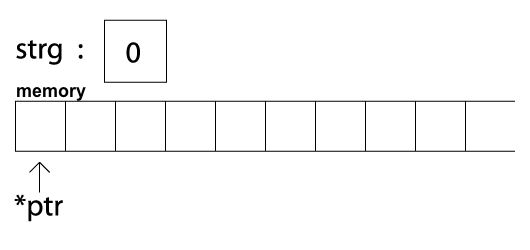
\includegraphics[width=0.6\textwidth]{./images/expl-rna.png}
    \caption{Ilustração das estruturas de armazenamento do \emph{RNA}}
    \label{fig:expl-rna}
\end{figure}

As 16 instruções implementadas correspondem às seguintes instruções em C:

\begin{enumerate}
	\item \textbf{AUG}: \verb$int main() {$
	\item \textbf{UAA}: \verb$} // end_main$
	\item \textbf{UGG}: \verb$strg=0;$
	\item \textbf{AAA}: \verb$++strg;$
	\item \textbf{AAC}: \verb$--strg;$
	\item \textbf{GCA}: \verb$strg=*ptr;$
	\item \textbf{ACA}: \verb$ptr=&memory[strg];$
	\item \textbf{CCA}: \verb$scanf(“%d”, ptr);$
	\item \textbf{CUA}: \verb$printf(“%c”, *ptr);$
	\item \textbf{AGA}: \verb$*ptr+=memory[strg];$
	\item \textbf{AGC}: \verb$*ptr*=memory[strg];$
	\item \textbf{CAA}: \verb$*ptr-=memory[strg];$
	\item \textbf{CAC}: \verb$*ptr/=memory[strg];$
	\item \textbf{GAA}: \verb$*ptr=*ptr==memory[strg]?1:0;$
	\item \textbf{GAC}: \verb$while(*ptr) {$
	\item \textbf{UAC}: \verb$} // end_while$
\end{enumerate}

Com relação a implementação em C da linguagem\footnote{http://esolangs.org/wiki/RNA}, foram encontrados alguns erros que foram corrigidos a fim de permitir o teste de programas em RNA. Abaixo, segue o \emph{diff} do que foi modificado com relação à implementação original.

\lstinputlisting[frame=single,breaklines=true,basicstyle=\tiny]{files/diff_rna.txt}

A implementação do interpretador \emph{RNA} com as correções pode ser encontrada junto com o código final, para permitir a realização de testes.
